\section{Umsetzung}

\subsection{Verwendete Softwarehilfsmittel}
    \begin{itemize}
        \item jReality~\cite{jreality}
        \item polymake~\cite{polymake}
        \item maven~\cite{maven}
        \item jUnit
    \end{itemize}
    
\subsection{Softwarearchitektur}
     \begin{figure}[tbh]
            \centering
            \fbox{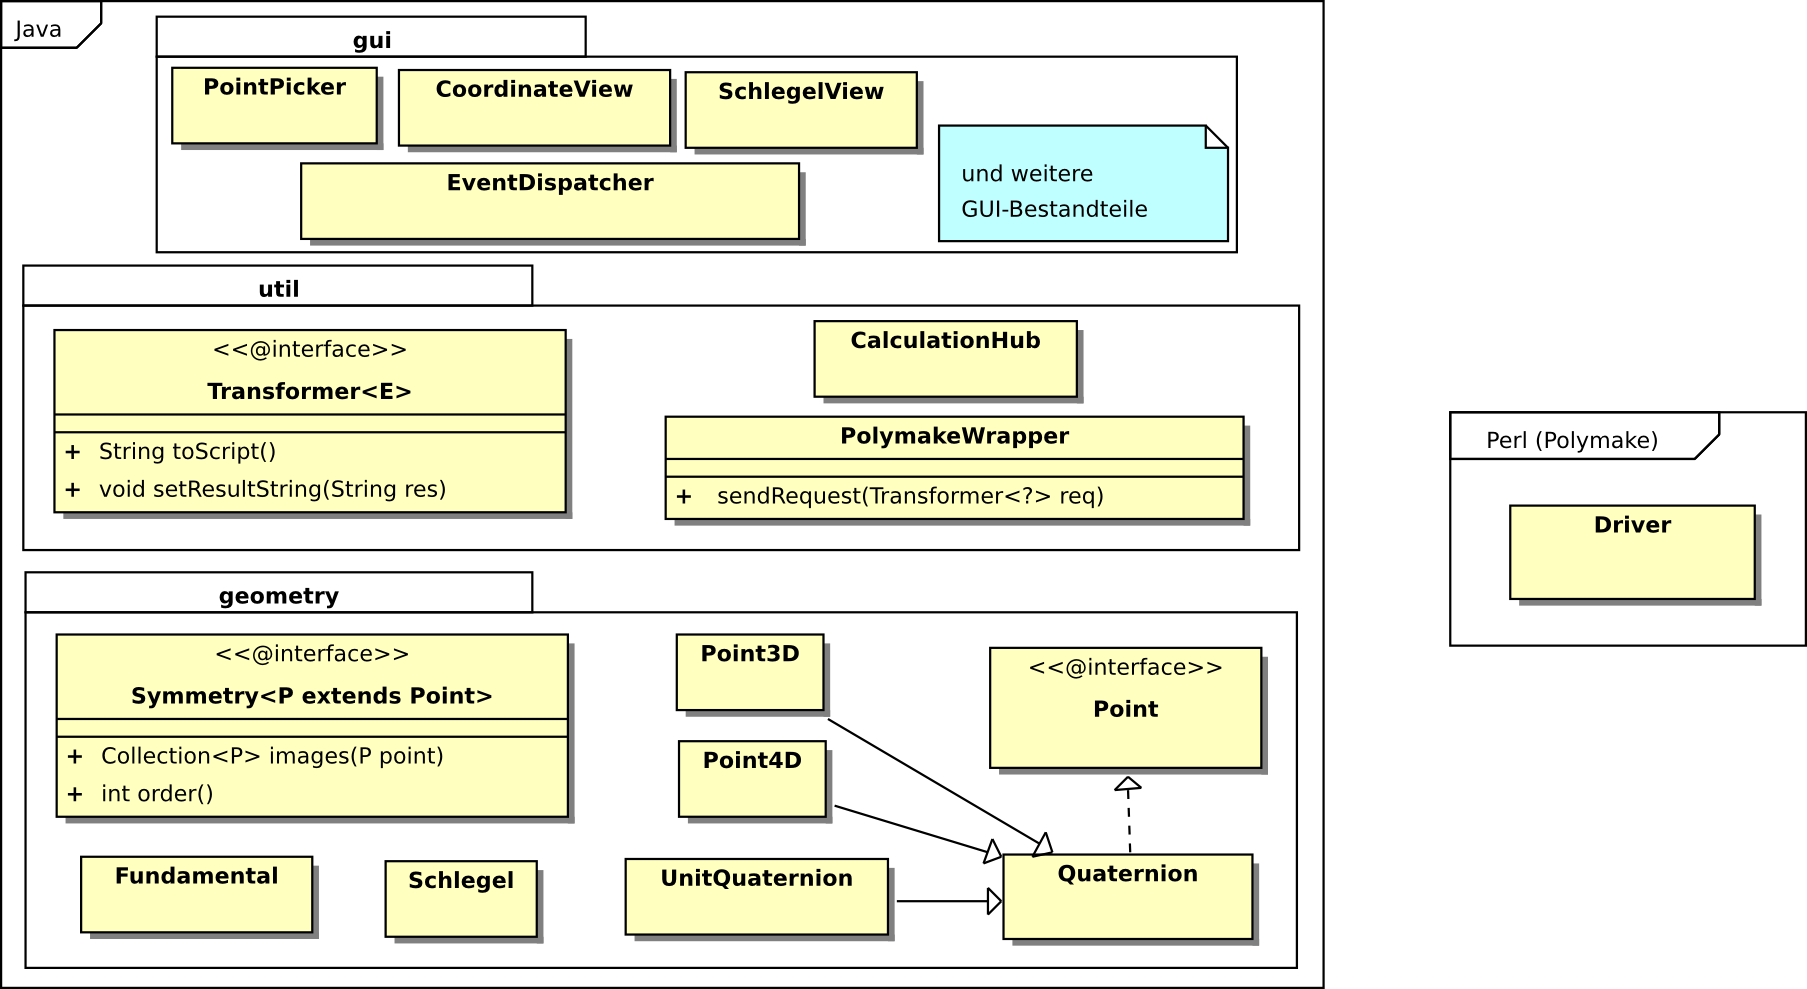
\includegraphics[width=0.7\textwidth]{img/architecture}}
            \caption{Grobübersicht über die Architektur des Projekts}
        \end{figure}
    \begin{itemize}
        \item Eventsystem (Eventstruktur)
        \item Pipeline (Symmetriegruppe wählen, Fundamentalbereich berechnen und anzeigen, Punkt im Fundamentalbereich auswählen, Punkt unter Symmetrien abbilden, konvexe Hülle Berechnen, im 3--dimensionalen konvexe Hülle anzeigen/im 4--dimensionalen Schlegeldiagram berechnen, anzeigen)
        \item GUI
    \end{itemize}
    \subsubsection{Eventssystem}
        \begin{figure}[tbh]
            \centering
            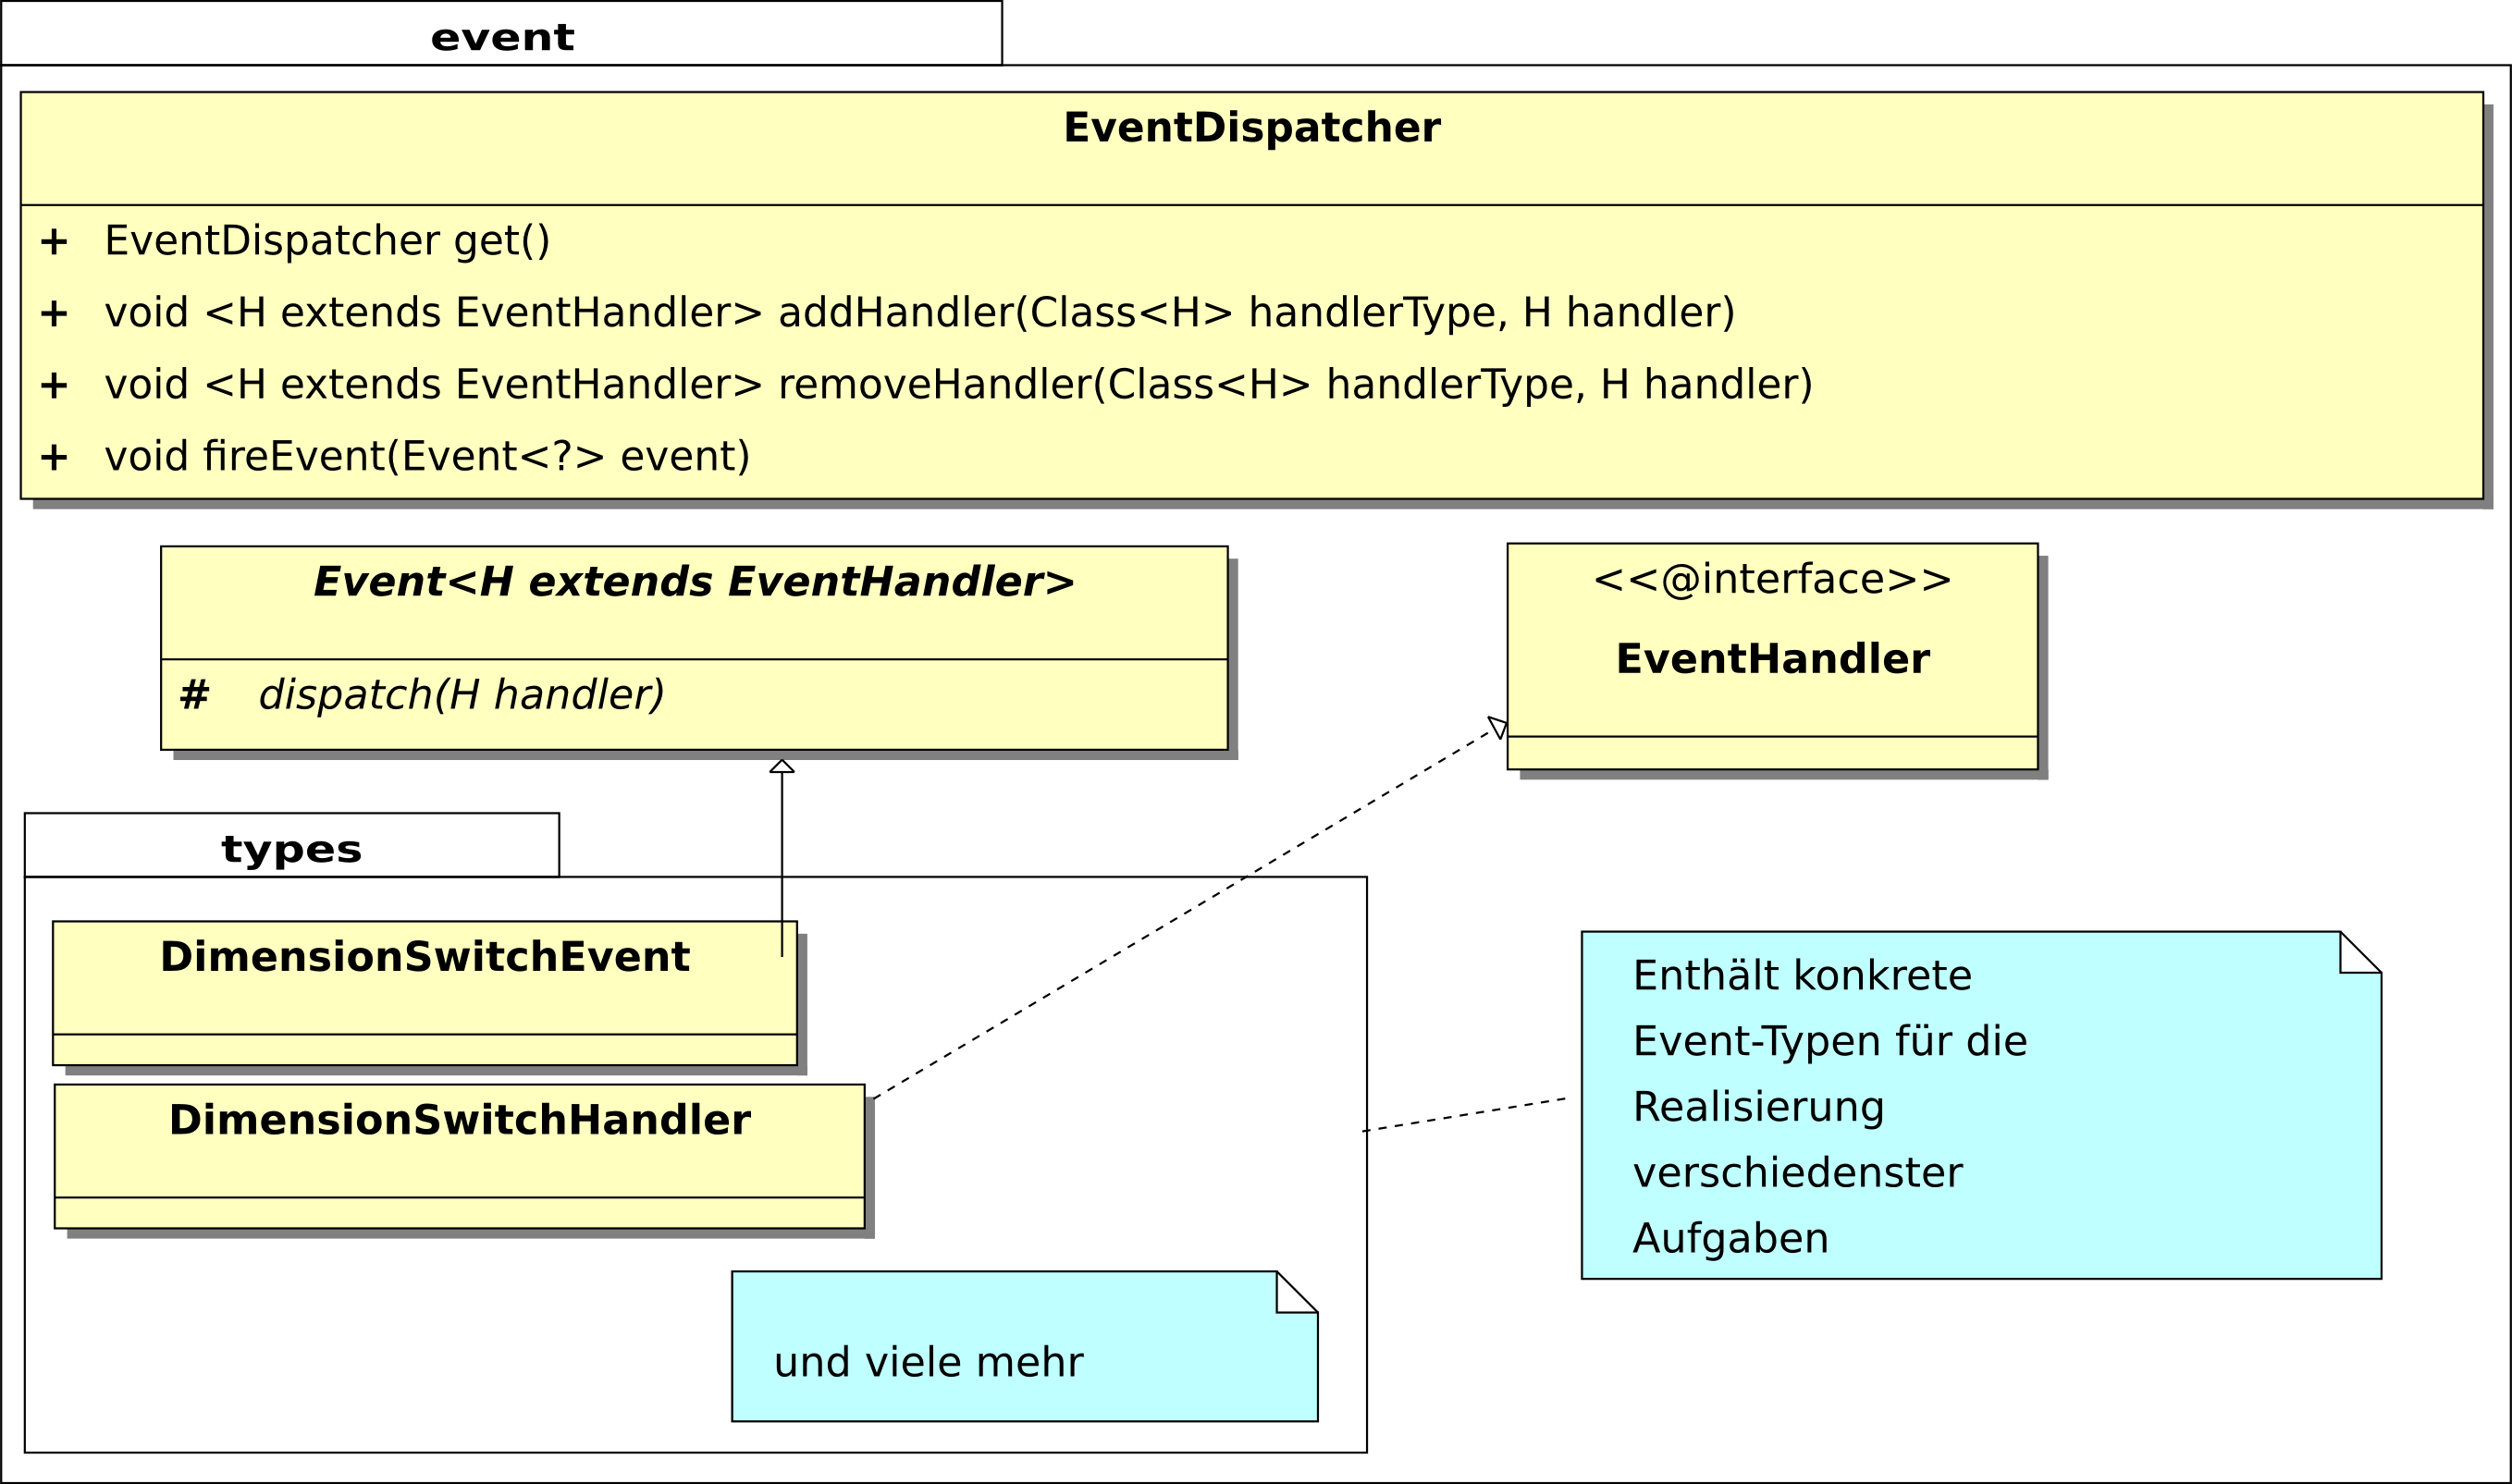
\includegraphics[width=0.8\textwidth]{img/event_classdiagram2}
            \caption{Klassendiagramm des Eventsystems}
        \end{figure}
        \subsubsection*{Events}
            Events sind konkrete Reaktionen auf bestimmte Ereignisse und enthalten entsprechende Kontextinformationen. Alle Typen von Events erben von der abstrakten Klasse Event<H extends EventHandler>. Klassen, die auf bestimmte Event-Typen reagieren wollen, implementieren das zum Event zugeordnete Interface EventHandler.

            Jede Klasse, die Events abfeuern möchte, muss einen Verweis auf den EventDispatcher besitzen. Ein Singleton von diesem Dispatcher kann mittels EventDispatcher.get() eingeholt werden. Soll ein konkretes Event e gefeuert werden, wird dies via dispatcher.fireEvent(e) erledigt. Alle Klassen, die sich vor dem Feuern eines Events via dispatcher.addHandler(eventType, handler) registriert haben, werden die Events vom Typ eventType erhalten. Der Event-Typ sollte, via Konvention, durch KonkretesEvent.TYPE gegeben sein (wobei KonkretesEvent eine Implementieren von Event ist).
        \subsubsection*{Eventimplementierung}
            Event-Typen werden durch Anlegen einer Event-Klasse und einer EventHandler-Klasse hinzugefügt.

            Das EventHandler-Template ist
            
            \begin{code}
                import pointGroups.gui.event.EventHandler;

                public interface ConcreteHandler
                    extends EventHandler
                {
                    public void onConcreteEvent(final ConcreteEvent event);
                }
            \end{code}

            Das Event-Typ-Template ist

            \begin{code}            
                import pointGroups.gui.event.Event;

                public class ConcreteEvent
                    extends Event<ConcreteHandler>
                {
                    public final static Class<ConcreteHandler> TYPE =
                        ConcreteHandler.class;

                    @Override
                    public final Class<ConcreteHandler> getType() {
                        return TYPE;
                    }

                    @Override
                    protected void dispatch(final ConcreteHandler handler) {
                        handler.onConcreteEvent(this);
                    }
                } 
            \end{code}
            
            wobei Concrete durch konkrete Namen ersetzt werden kann.
            
        \subsubsection*{Implementierte Events}
            Eventuelle Auflistung aller oder nur einzelner.
                
\subsection{Fancy name}
    \begin{itemize}
        \item Symmetriegruppen (Berechnung mittels Generatoren, hart kodiert, Darstellung/Repräsentation)
        \item Fundamentalbereich (Berechnung, Darstellung/Repräsentation)
    \end{itemize}
    
    \subsubsection{Symmetriegruppen}
    \subsubsection{Fundamentalbereich}
         In Abschnitt \ref{fundamentalbereich} wurde in Definition \ref{fundamentalbereich:voronoi} der Voronoi-Fundamentalbereich beschrieben. Wir wollen eine dieser Zellen
         nehmen und Visualisieren. Da wir einen Abschnitt der $S^3$ nicht leicht visualsieren können, benötigen wir zunächst eine Projektion das Vornoi-Fundamentalbereiches auf
         eine $\mathbb{R}^3$ Ebene.
        \subsubsection*{Idee}
            Wir lassen zunächst die Gruppe auf ein Ausgezeichnetes Element $x$ wirken.

            Als erstes Berechnen wir die Voronoi - Zelle für $x$ bezüglich des Orbits von $x$. Alle Punkte die dort drinnen liegen sind Elemente von $S^3$. Da die Gruppe symmet          risch ist, können wir nicht zwei Elemente aus dem selben Orbit haben, da der zweite Punkt näher an einem anderen Element aus $G \rhd x$ liegen müsste.

         Das einzig wichtige an diesem Punkt ist, dass $x$ nicht auf einer Rotationasachse oder Spiegelebene befindet, da sonst die Voronoizellen zu groß ausfallen.

         Haben wir diese Zelle, nehmen wir eine beliebige Ebene, die tangential auf dem Kugelsegment ist und projezieren darauf. Die spezielle Ebene, die wir wählen
         ist die Ebene $h \, : \, [t - x] \cdot x = 0$ in Normalendarstellung, da wir wissen, dass $x$ auf der Kugeloberfläche im Kreissegment liegt und $x$ auch ein
          Normalenvektor ist.
            
        \subsubsection*{Umsetzung}
         Eine Voronoizelle von $x$ für eine Menge von Sites $S$ ist definiert als 
         $$ VC(x) = \bigcap_{s \in S \setminus \{ x \}} h^+_{x,s}$$
         Wobei $h^+_{x,s}$ der Halbraum ist, der rechts von der Hyperebene liegt, die zu $x$ und $y$ in jedem Punkt den selben Abstand hat.\\

         Polymake hat die Möglichkeit ein Polytope, das die Voronoizelle ja ist, gerade über den Schnitt von Halbräumen zu definieren. Dies geht über

         \begin{code}
            new Polytope(INEQUALITIES=>\$hyperplanes)
         \end{code}

         wobei \$hyperplanes eine Menge von Hyperebenen ist. Falls ein affines Polytope vorliegt, wie in unserem Fall in der Ebene $h$, die wie im letzten Abschnitt
         definiert ist, können wir auch dies mit in die Erzeugung eingeben mittels

         \begin{code}
            new Polytope(INEQUALITIES=>\$hyperplanes, EQUATIONS=>{h})
         \end{code}

         und haben so $VC(x)$ berechnet. Da die konkrete Berechnung über den Schnitt von allen Hyperebenen zu lange dauert, filtern wir die in frage kommenden Hyperebenen vor
         über die Nachbern des Voronoi Diagrams. Dummerweise konnten wir nicht ermitteln, wie man in Polymake sich direkt eine Voronoizelle ausgeben lassen kann und
         haben daher diesen Umweg gewählt.\\

         Haben wir nun das Polytope in der Ebene, müssen wir zur Darstellung in $n-1$ Dimensionen noch eine geeignete Basis berechnen, so dass wir
         die Eckpunkte des Polytopes durch $n-1$ Koordinaten darstellen können. Wir wissen schon, dass $x$ senkrecht auf der Ebene steht, also für unsere Darstellung 
         unerheblich ist. Wir berechnen eine Orthonormalbasis für die Ebene mit $x$ als erstem Basisvektor. Nun können wir leicht eine Basiswechselmatrix angeben,
         da wir ja die Bilder der neuen Basis in der alten kennen. Darüber hinaus ist diese Matrix orthogonal -- da die Spalten ja eine orthogonal Basis waren -- und
         kann daher durch transponieren invertiert werden.

         Wir haben nun also zwei Matrizen um beide Darstellungen in einander umzurechnen. In der neuen Basis können wir nun die erste Komponente weg lassen,
         da diese nach Projektion nur genullt wird und haben so eine Darstellung in $n-1$ Dimensionen.

         Beim zurückrechnen müssen wir uns nur erinnern, dass wir uns in einer affinen Ebene mit Stützvektor $x$ befinden.

        \subsubsection*{Berechnung}

         Die Hyperebenen Definition in Polymake hat die Darstellung
         $$
            h \, : \, [a_0, ..., a_n] \rightsquigarrow a_0 + a_1 x_1 + \cdots + a_n x_n = 0
         $$
         und Halbräume ebenso mit $\geq 0$.\\

         Die Halbräume für unser Polytope genügen der Gleichung
         $$
            t \cdot (x - s) \geq 0 \Leftrightarrow 0 + (x_1-s_1)\cdot t_1 + \cdots + (x_n -s_n)t_n \geq 0
         $$
         wobei $x$ der gewählte Vektor war und $s \not x$ aus dem Orbit von $x$ stammt.

         Damit können wir alle Halbräume aus dem Orbit berechnen. Die affine Ebene genügt der Gleichung
         $$
            (t - x) \cdot x = 0 \Leftrightarrow - \left( \sum_{i=1}^n x_i^2 \right) + t_1 x_1 + \cdots t_n x_n = 0
         $$
         und kann auch leicht erstellt werden. Um an unser Polytope heran zu kommen, benutzen wir das folgende Polymake-Script

         \begin{code}
            my \$poly = new Polytope(INEQUALITIES=>\$hyperplanes, EQUATIONS=>\$affine);
            print \$poly->VERTICES;
            print \$poly->EDGES;
            print \$poly->FACETS;
         \end{code}

         Mit diesen Ergebnissen können wir nun die Basiswechselmatrizen berechnen und so die Vertices umrechnen. Das Object Fundamental ist somit
         eine Sammlung dieser Eigenschaften.

         \begin{code}
            public interface Fundamental {
               public double[][] getVertices();
               
               public Edge<Integer,Integer>[] getEdges();

               public double[] revertPoint(double[] point);

               public boolean inFundamental(double[] point);
            }
         \end{code}
         
         Die ersten beiden Funktionen sind selbst erklärend. Die dritte methode \emph{revertPoint} nimmt einen Punkt in $\mathbb{R}^{n-1}$ und
         liftet ihn auf die Oberfläche der $S^{n-1}$ zurück. Die letzte Methode überprüft, ob ein angegebener Punkt überhaupt in der Voronoizelle lag.
         Diese Methode wird bei der anzeige beötigt um bei der Punktauswahl keine Punkte außerhalb das Polytops zuzulassen.\\

         Das ganze ist ein interface, da wir als Fallback-case, falls die Berechnung das Fundamentalbereichs einmal fehl schlägt immer noch 
         den Bereich $S^{n-2}$ benutzen können. Dies ist kein Fundamentalbereich, da wir alle Orbite mehrfach treffen, allerdings werden wir außer im Falle
         der Identität wirklich jeden Orbit mindestens einmal treffen.
